\subsection{Optimization of Compiler-Generated OpenCL CNN Kernels and runtime for FPGAs}
\subsubsection{Triển khai mạng đầu cuối}
Sơ đồ luồng biên dịch được thể hiện ở hình bên dưới:
\begin{figure}[!h]
    \centering
    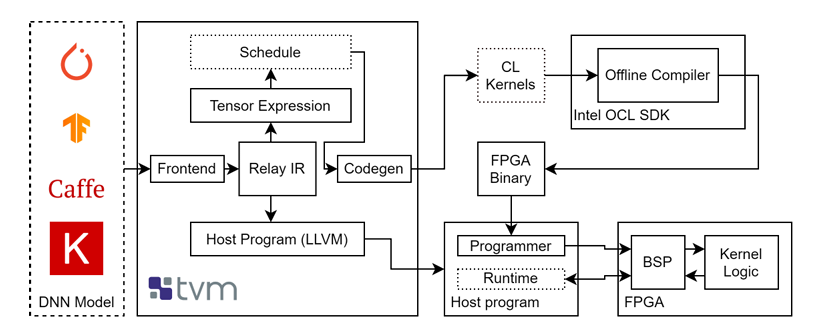
\includegraphics[width=\textwidth]{Images/CNNAccelerator/OptimizingCompiler-GeneratedOpenCLforCNNs/compilation_flow.png}
    \vspace{10pt} % Thay đổi giá trị 10pt theo nhu cầu
    \caption{Sơ đồ luồng biên dịch}
\end{figure}
\begin{itemize}
    \item Đầu vào: Mô hình CNN từ các framework ML khác nhau.
    \item TVM - một công cụ biên dịch tối ưu hóa cho học sâu, chuyển đổi mô hình thành biểu diễn trung gian (Relay IR).
    \item Biên dịch: TVM tạo mã OpenCL C từ Relay IR, sử dụng các hàm tính toán và lịch biểu được tối ưu hóa từ TVM Operator Inventory (TOPI).
    \item Tổng hợp: Intel OpenCL SDK tổng hợp mã OpenCL C thành phần cứng FPGA.
    \item Thực thi: Luồng dữ liệu được tạo trên FPGA để thực thi mô hình CNN.
\end{itemize}
Luồng biên dịch hỗ trợ hai chế độ thực thi: thực thi theo đường ống (pipelined) và thực thi gấp (folded).
\begin{itemize}
    \item Thực thi theo đường ống: Các bản đồ đặc trưng đầu ra được chuyển giữa các kernel bằng cách sử dụng các kênh OpenCL.
    \item Thực thi gấp: Các kernel được tham số hóa (hình dạng tensor đầu vào/đầu ra động) được sử dụng lại cho nhiều lớp trong mạng, tiêu thụ ít tài nguyên FPGA hơn so với thiết kế đường ống đầy đủ.
\end{itemize}
\subsubsection{Tối ưu hóa kernel OpenCL}
Các vấn đề với kernel OpenCL được tạo bởi trình biên dịch TVM:
\begin{itemize}
    \item Sử dụng bộ nhớ toàn cục không hiệu quả: Dẫn đến hiệu suất thấp do băng thông bộ nhớ toàn cục hạn chế.
    \item Sử dụng logic không hiệu quả: Dẫn đến việc sử dụng tài nguyên cao, làm cho các thiết kế lớn hơn không thể tổng hợp được.
    \item Tính song song thấp: Dẫn đến hiệu suất kém.
\end{itemize}
Các biện pháp tối ưu hóa được đề xuất:
\begin{itemize}
    \item Đọc coalesced: Kết hợp nhiều lần đọc nhỏ thành các lần đọc rộng hơn, cải thiện việc sử dụng băng thông bộ nhớ toàn cục.
    \item Lặp unrolling: Nhân rộng thân vòng lặp để tăng tính song song.
    \item Lặp fusion: Kết hợp nhiều vòng lặp thành một vòng lặp để giảm chi phí điều khiển vòng lặp và cải thiện cục bộ bộ nhớ cache.
    \item Di chuyển mã bất biến: Di chuyển các tính toán bất biến ra khỏi vòng lặp để giảm chi phí tính toán.
    \item Ghi bộ nhớ cache: Ghi kết quả trung gian vào bộ nhớ cục bộ để giảm truy cập bộ nhớ toàn cục.
    \item Kênh: Sử dụng kênh OpenCL để truyền dữ liệu giữa các kernel, giảm chi phí truyền dữ liệu bộ nhớ toàn cục và tăng tính song song.
    \item Kernel Autorun: Cho phép các kernel không có trọng số hoặc độ lệch thực thi ngay khi bộ đệm đầy, tăng tính song song.
    \item Thực thi đồng thời: Sử dụng nhiều hàng đợi lệnh để cho phép các kernel chạy song song, tăng hiệu suất.
    \item Kernel được tham số hóa: Nhóm và tham số hóa các kernel tương tự để chúng có thể được sử dụng lại trên toàn mạng, giảm mức sử dụng tài nguyên.
    \item Tối ưu hóa hoạt động dấu phẩy động: Sử dụng các tối ưu hóa do Intel OpenCL SDK cung cấp để cải thiện hiệu suất của các hoạt động dấu phẩy động.
\end{itemize}
Các phương pháp tối ưu hóa và khả năng áp dụng của chúng được thể hiện ở hình bên dưới.
\begin{figure}[!h]
    \centering
    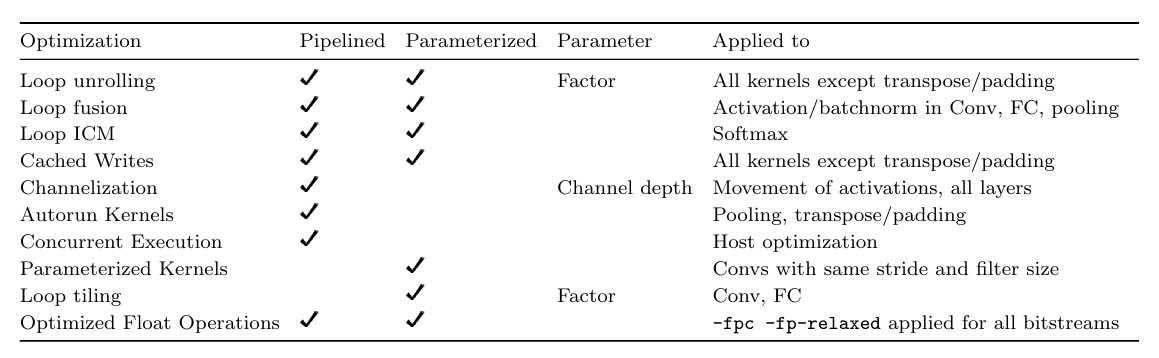
\includegraphics[width=\textwidth]{Images/CNNAccelerator/OptimizingCompiler-GeneratedOpenCLforCNNs/optimization_summary.png}
    \vspace{10pt} % Thay đổi giá trị 10pt theo nhu cầu
    \caption{Các phương pháp tối ưu hóa và khả năng áp dụng của chúng}
\end{figure}
\subsubsection{Triển khai}
\paragraph{Schedule Optimization}
\begin{itemize}
    \item Lớp Convolution: Schedule được tối ưu hóa bao gồm unrolling vòng lặp giảm, tiling dọc theo kênh FM đầu vào và cột FM đầu ra và unrolling các vòng lặp bên trong.
    \item Lớp fully-connected (FC): Lịch biểu được tối ưu hóa liên quan đến việc khai thác vòng lặp bên trong để tối đa hóa việc sử dụng bộ nhớ toàn cục và unrolling vòng lặp bên trong.
    \item Lớp Softmax: Lịch biểu được tối ưu hóa bao gồm việc kết hợp các vòng lặp để tính toán giá trị tối đa và tổng hàm mũ.
\end{itemize}
\paragraph{Custom Host Code}
Một chương trình máy chủ OpenCL C/C++ được triển khai bên ngoài TVM để hỗ trợ các tối ưu hóa không được hỗ trợ trong mã tạo máy chủ TVM.
\paragraph{Symbolic Shape Execution}
Tính năng này được sử dụng để nhóm việc thực thi các phép chập có cùng bước và kích thước bộ lọc vào cùng một kernel, cho phép sử dụng lại kernel và giảm mức sử dụng tài nguyên.
\subsubsection{Đánh giá}
\paragraph{Phương pháp}
\begin{itemize}
    \item Ba mạng CNN (LeNet-5, MobileNetV1 và ResNet-18/34) được triển khai trên ba nền tảng FPGA (Intel Arria 10, Stratix 10 MX và Stratix 10 SX).
    \item Hiệu suất được so sánh với các triển khai được tối ưu hóa cao trên CPU và GPU.
    \item Các chỉ số hiệu suất bao gồm FPS (Frames per second), GFLOPS (Floating-point operations per second) và mức sử dụng tài nguyên.
\end{itemize}
\paragraph{Nền tảng}
Thực hiện thí nghiệm với 3 nền tảng sau:
\begin{itemize}
    \item FPGA: Intel Arria 10 GX, Stratix 10 SX và Stratix 10 MX.
    \item CPU: Intel Xeon Platinum 8280.
    \item GPU: NVIDIA GTX 1060.
\end{itemize}
\paragraph{Hiệu suất suy luận}
\textbf{LeNet-5}:
Kết quả được hiển thị ở bên dưới:
\begin{figure}[!h]
    \centering
    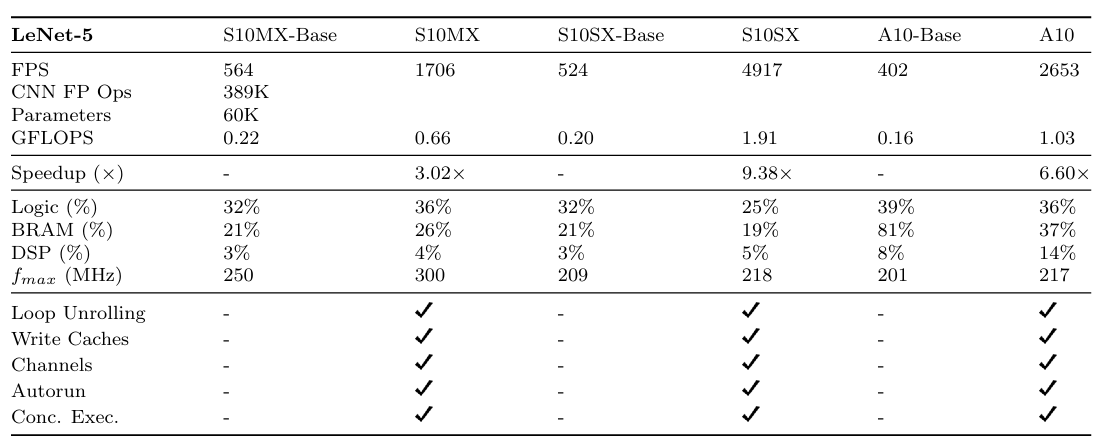
\includegraphics[width=\textwidth]{Images/CNNAccelerator/OptimizingCompiler-GeneratedOpenCLforCNNs/lenet5_inference.png}
    \vspace{10pt} % Thay đổi giá trị 10pt theo nhu cầu
    \caption{Kết quả khi hiện thực LeNet-5}
\end{figure}
\begin{itemize}
    \item FPGA đạt hiệu suất từ 1.59$\times$ đến 4.57$\times$ so với TF-CPU, 0.73$\times$ đến 2.10$\times$ so với TVM-1T và 1.06$\times$ đến 3.07$\times$ so với TF-cuDNN.
    \item Kết luận: Các bitstream FPGA được tối ưu hóa mang lại hiệu năng vượt trội so với CPU và cạnh tranh với GPU.
\end{itemize}
\textbf{MobileNetV1}
Kết quả được hiển thị ở bên dưới:
\begin{figure}[!h]
    \centering
    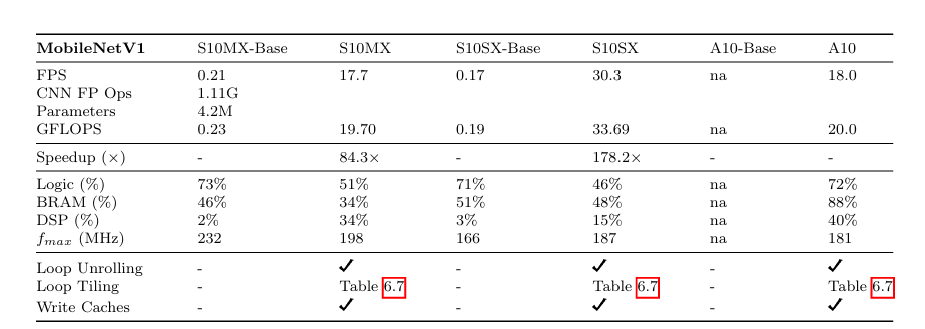
\includegraphics[width=\textwidth]{Images/CNNAccelerator/OptimizingCompiler-GeneratedOpenCLforCNNs/mobilenet.png}
    \vspace{10pt} % Thay đổi giá trị 10pt theo nhu cầu
    \caption{Kết quả khi hiện thực MobileNetV1}
\end{figure}
\begin{itemize}
    \item FPGA đạt hiệu suất từ 0.82$\times$ đến 1.40$\times$ so với TF-CPU, 1.13$\times$ đến 1.94$\times$ so với TVM-1T và chậm hơn từ 0.41$\times$ đến 0.69$\times$ so với TF-cuDNN.
    \item Kết luận: FPGA mang lại hiệu năng cạnh tranh với CPU và chậm hơn GPU, hiệu suất bị giới hạn bởi việc sử dụng DSP thấp và hiệu suất của các lớp khác.
\end{itemize}
\textbf{ResNet}
Kết quả được hiển thị ở bên dưới:
\begin{figure}[!h]
    \centering
    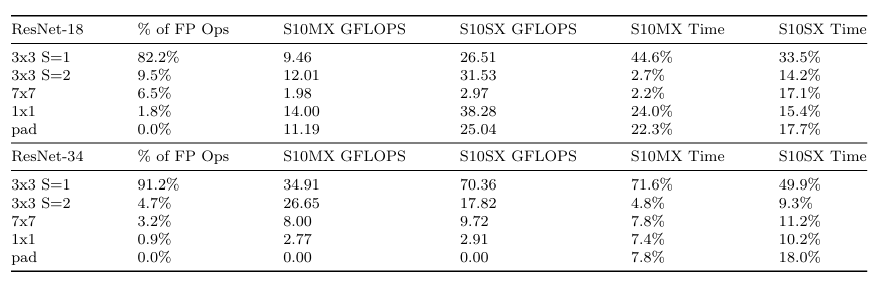
\includegraphics[width=\textwidth]{Images/CNNAccelerator/OptimizingCompiler-GeneratedOpenCLforCNNs/resnet.png}
    \vspace{10pt} % Thay đổi giá trị 10pt theo nhu cầu
    \caption{Kết quả khi hiện thực ResNet}
\end{figure}
\begin{itemize}
    \item FPGA chậm hơn CPU và GPU.
    \item Kết luận: Hiệu suất bị giới hạn bởi việc sử dụng DSP thấp và hiệu suất của các lớp khác.
\end{itemize}
\subsubsection{Hạn chế}
\begin{itemize}
    \item Sử dụng khối DSP thấp: Việc triển khai bị giới hạn bởi khả năng sử dụng DSP tối đa đạt được, đặc biệt là đối với các mạng lớn hơn.
    \item Suy giảm Fmax: Việc lát gạch và trải cuộn vòng lặp có thể dẫn đến suy giảm fmax do tăng độ phức tạp của việc định tuyến.
    \item Hiệu suất của các lớp khác: Hiệu suất của các phép cuộn 3x3 chiều sâu, đệm, softmax, và các lớp dày đặc hiện đang giới hạn hiệu suất tổng thể.
\end{itemize}